\documentclass[a4paper, itemph]{oblivoir}
\setmainhangulfont{NANUMMYEONGJO.TTF}[BoldFont={NANUMMYEONGJOEXTRABOLD.TTF}]
\usepackage[english]{babel}
\usepackage[utf8x]{inputenc}
\usepackage[T1]{fontenc}
%% Sets page size and margins
\usepackage[a4paper,top=3cm,bottom=2cm,left=3cm,right=3cm,marginparwidth=2cm]{geometry}

\usepackage{indentfirst}

%% Useful packages
\usepackage{amsfonts}
\usepackage{amsmath, mathtools}
\usepackage{graphicx}
\usepackage{subcaption}
\usepackage[colorinlistoftodos]{todonotes}
\usepackage{amssymb}
\usepackage{amsthm}
\usepackage{tikz}
\usepackage{pgfplots}
\usepackage{filecontents}

%Extravaganza
\newtheorem{thm}{Theorem}[subsection]
\newtheorem{lem}{Lemma}[subsection]
\newtheorem{cor}{Corollary}[subsection]
\newcommand{\overbar}[1]{\mkern 1.5mu\overline{\mkern-1.5mu#1\mkern-1.5mu}\mkern 1.5mu}
\theoremstyle{definition}
\newtheorem{defn}{Definition}[subsection]
\newtheorem{rem}{Remark}[subsection]

\begin{filecontents}{reverse.csv}
     -10        -4.286      -4.300e-6
     -9         -4.068      -4.082e-6
     -8         -3.988      -4.002e-6
     -7         -3.678      -3.691e-6
     -6         -3.695      -3.708e-6
     -5         -3.634      -3.646e-6
     -4         -3.669      -3.681e-6
     -3         -3.291      -3.302e-6
     -2         -2.972      -2.981e-6
     -1         -2.611      -2.620e-6
     -0.9       -2.532      -2.541e-6
     -0.8       -2.502      -2.511e-6
     -0.7       -2.383      -2.391e-6
     -0.6       -2.406      -2.414e-6
     -0.5       -2.345      -2.353e-6
     -0.4       -2.209      -2.217e-6
     -0.3       -2.173      -2.180e-6
     -0.2       -2.133      -2.140e-6
     -0.1       -1.999      -2.006e-6
\end{filecontents}

\begin{filecontents}{forward.csv}
     0.1        0.075e-3    -2.590
     0.2        0.762e-3    -0.272
     0.3        4.297e-3    1.458
     0.4        20.302e-3   3.012
     0.5        203.92e-3   5.318
     0.6        869.86e-3   6.768
     0.7        6.8132      8.827
     0.8        19.8267     9.895
\end{filecontents}

\begin{document}
\title{기초전자회로 및 실험: Lab \#01}
\author{서울대학교 전기$\cdot$정보공학부 2018-12602 이준협}
\date{April 3, 2020}
\maketitle

\section{Diode I-V Characteristics Under Forward and Reverse Bias}
\begin{center}
\scalebox{0.5}{
\begin{tikzpicture}
  \begin{axis}[
  /pgf/number format/set thousands separator = {},
    xlabel = $V_D\mathrm{[V]}$,
    ylabel = $I_D\mathrm{[mA]}$,
    ]
    \addplot [only marks, black] table[x index=0,y index=2,header=false] {reverse.csv};
    \addplot [no markers, red] gnuplot [raw gnuplot] { % "raw gnuplot" allows us to use arbitrary gnuplot commands
            f(x) = a*(exp(x/b)-1); % Define the function to fit
            a=1e-6; b=26e-3; % Set reasonable starting values here
            fit f(x) 'reverse.csv' u 1:3 via a,b; % Select the file, the columns (indexing starts at 1) and the variables
            plot [x=-10:0] f(x); % Specify the range to plot
    };
    \legend{$I_D$}
  \end{axis}
\end{tikzpicture}
}\quad
\scalebox{0.5}{
\begin{tikzpicture}
  \begin{axis}[
  /pgf/number format/set thousands separator = {},
    xlabel = $V_D\mathrm{[V]}$,
    ylabel = $I_D\mathrm{[mA]}$,
    ]
    \addplot [only marks, black] table[x index=0,y index=1,header=false] {forward.csv};
    \addplot [no markers, red] gnuplot [raw gnuplot] { % "raw gnuplot" allows us to use arbitrary gnuplot commands
            f(x) = a*(exp(x/b)-1); % Define the function to fit
            a=1.75e-5; b=55.58e-3; % Set reasonable starting values here
            fit f(x) 'forward.csv' u 1:2 via a,b; % Select the file, the columns (indexing starts at 1) and the variables
            plot [x=0:0.8] f(x); % Specify the range to plot
    };
  \end{axis}
\end{tikzpicture}
}\quad
\scalebox{0.5}{
\begin{tikzpicture}
  \begin{axis}[
  /pgf/number format/set thousands separator = {},
    xlabel = $V_D\mathrm{[V]}$,
    ylabel = $\mathrm{ln}(I_D\times 10^6)$($I_D$ measured in Amps),
    ]
    \addplot [only marks, black] table[x index=0,y index=2,header=false] {forward.csv};
    \addplot [no markers, red] gnuplot [raw gnuplot] { % "raw gnuplot" allows us to use arbitrary gnuplot commands
            f(x) = a*x+b; % Define the function to fit
            a=40; b=-5; % Set reasonable starting values here
            fit f(x) 'forward.csv' u 1:3 via a,b; % Select the file, the columns (indexing starts at 1) and the variables
            plot [x=0:0.8] f(x); % Specify the range to plot
    };
  \end{axis}
\end{tikzpicture}
}
\end{center}

The first plot shows the current flowing through the diode in the case of reverse bias, which was calculated by dividing the voltage on the resistor connected in series by the resistance(0.99661[M$\Omega$]). One can see that the saturation current is in the nA range($=10^{-6}$[mA]), however the current does not saturate as in the red plot, which was estimated by gnuplot to fit the exponential model. Although fitting an exponential model is not a good idea, it is still true that despite the current seeming to saturate in the -7[V] to -4[V] range, the gradient increases when the voltage decreases further below -7[V]. This is an indication to the fact that the decay is certainly not exponential in the reverse bias region, as the gradient must decrease(the current must decrease more slowly) in the case of exponential decay.

The second plot shows the current flowing through the diode in forward bias. The cut-in voltage is shown to be around 0.8[V], and the slope is not infinity; the ideal diode model is not adequate to predict this behavior. The current is then plotted in log scale in the third plot, then fitted by a linear model to further confirm the exponential model. The linear model can be applied, since $\mathrm{ln}(I_S\exp(V_D/V_T)\times10^6)=V_D/V_T+\mathrm{ln}(I_S\times10^6)$, when $V_D$ is in Volts, $I_S$ in Amperes. The line is calculated to be $y=17.9912x-4.044$, so $V_T\approx 55.58$[mV] and $I_S\approx 17.53$[nA]. The exponential model in the forward bias region seems to fit well, since the linear model in log scale fits with an $R^2$ of nearly 99\%, however the values of $V_T$ and $I_S$ are strange. $V_T=kT/e$ is approximately $26$[mV] in 300[K], however the experimental value is more than double that value, which seems to imply a temperature of 600[K]. Also, the value of $I_S$ is much higher than measured in the reverse bias region, which generally stayed within 2[nA] to 4[nA]. This means that the current seems to flow about 4 times better in forward bias conditions. 
\section{Reasons for the Discrepancies with Theoretical Prediction}

Before discussing the theoretical reasons why the current in forward and reverse conditions do not meet the expectations of the exponential model, we will first go over possible errors made while measuring the current. The input impedance of the DMM4020 in the 200[mV] range is about 10[G$\Omega$], as specified in the datasheet of the multimeter, so it cannot change the voltage of the 1[M$\Omega$] resistor by more than 0.01\%. Moreover, the burden voltage of the ammeter in the 200[$\mu$A] range is less than 5[mV], which is less than 5\% of the 0.1[V] increment in voltage given when measuring in forward bias conditions. The human error caused while moving the dial of the power supply couldn't have caused more than 0.01[V] error, since the fine dial of the power supply increments the voltage in segments less than 0.01[V]. Therefore, in reverse bias conditions, the y axis can differ by 0.01\%, the x axis can differ by 5\%, so still the current when the voltage is less than -7[V] is less than the currents in the -7[V] to -4[V] range; it is still not exponential. In the forward bias region, the slope in the third plot can be changed to no more than 10\%, since since the x axis can change maximum 0.01[V]. Since the estimated slope was about 18, the slope can be changed to maximum 19.8, which results in a $V_T$ of about 50.5[mV], which still does not fit the exponential model.

\begin{figure}[htb]
    \centering
    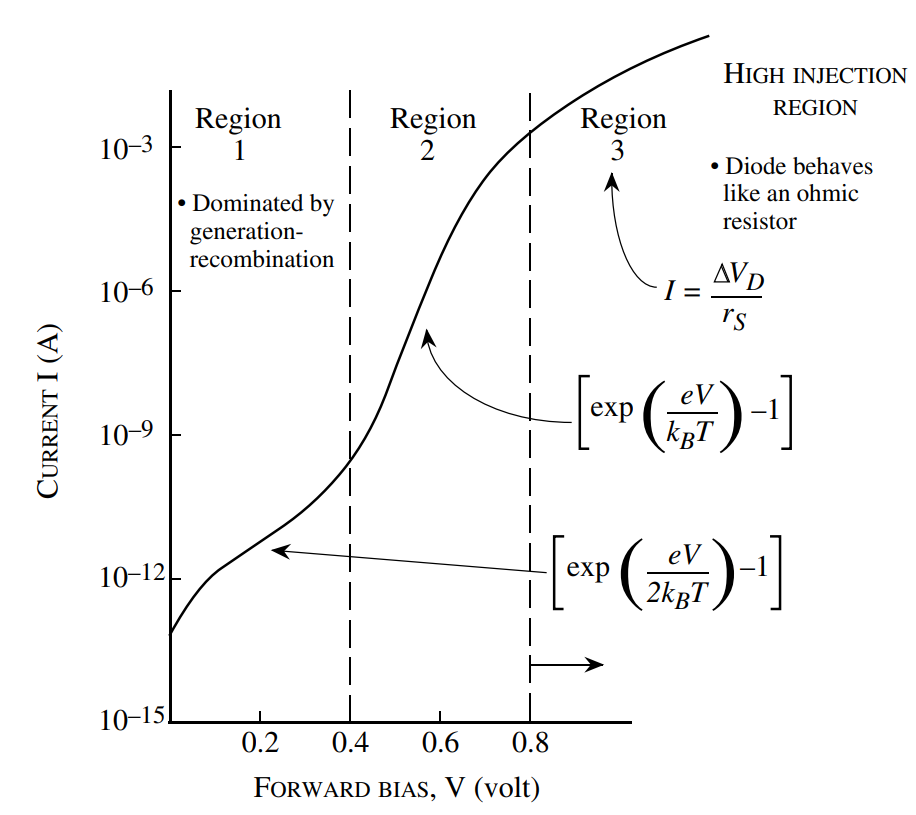
\includegraphics[width=0.5\linewidth]{nonideal.PNG}
    \caption{Current flowing through diodes in forward diode conditions. Source: Figure 4.14 in U. K. Mishra and J. Singh, \textit{Semiconductor Device Physics and Design}. Dordrecht: Springer, 2008, p.169.}
\end{figure}

A quick overview of the methods of measurement showed that measurement errors are not enough to explain the discrepancies with the equation $I_D=I_S(\exp(V_D/V_T)-1)$. The large $V_T$ and $I_S$ in the forward region is explained by the recombination current that is created because of the impurities that are introduced in the p-n junction, which forms a trap energy level between the conduction and valence energy band. This recombination current flows in the depletion region, which adds with the diffusion current that was originally thought to be the only reason of the diode current, and dominates the total current in low voltages. That is, it depends on how each diode is fabricated that changes the effective $I_S$ and $V_T$ of the forward current[1]. The equation is written as 
\[
I=I_0\left[\exp\left(\frac{eV}{kT}\right)-1\right]+I_{GR}^{\circ}\left[\exp\left(\frac{eV}{2kT}\right)-1\right]
\]
, when $I_0$ is the diffusion current and $I_{GR}^{\circ}$ is the recombination current, in equation 4.4.13[1]. This explains why the $V_T$ was measured to be about $\dfrac{2kT}{e}$ and $I_S$ was measured to be higher than $I_0$ in the reverse region.

In the reverse region, the same equation explains the behavior. The recombination current changes to the generation current, which is smaller than the recombination current in forward bias conditions. Also, the surface effects of the diodes near the contacts also lead to the current increasing when the reverse bias grows.
\begin{thebibliography}{}

\bibitem{1} U. K. Mishra and J. Singh, \textit{Semiconductor Device Physics and Design}. Dordrecht: Springer, 2008, pp. 163-177.

\end{thebibliography}

\end{document}
